%\begin{savequote}[75mm] 
%Nulla facilisi. In vel sem. Morbi id urna in diam dignissim feugiat. Proin molestie tortor eu velit. Aliquam erat volutpat. Nullam ultrices, diam tempus vulputate egestas, eros pede varius leo.
%\qauthor{Quoteauthor Lastname} 
%\end{savequote}

\chapter{Identification d'oeuvres}
\label{chap:similarite}
%%%%%%%%%%%%%%%%%%%%%%%%%%%%%%%%%%%%%%%%%%%%%%%%%%%%%%%%%
%														%
%		INTRODUCTION									%
%														%
%%%%%%%%%%%%%%%%%%%%%%%%%%%%%%%%%%%%%%%%%%%%%%%%%%%%%%%%%

Introduction :
Présenter l'identification d'oeuvres.
Mettre en avant le besoin d'apprentissage de similarité.
%
%Ce chapitre présente d'abord les motivations de cette recherche dans la section~\ref{sec:similaritemotivation}. Nous explorons ensuite en détail l'apprentissage de similarité~\ref{sec:similarite}. La section~\ref{sec:regions} présente l'apport de la détection de région dans la reconnaissance d'instance.

\section{Motivation}
\label{sec:similaritemotivation}


But : 
 - La recherche d'instance consiste à identifier les instances d'objets sur les image/vidéo.
 
 - La detection sur les images suffit si on considère qu'on peut detecter à quel moment déclencher la reco (cf geste)
 
 - La reco peut être fait par recherche d'image : en prenant les images les plus ressemblante. On va définir cette ressemblance en fonction de notre objectif. Notre objectif étant de savoir si tel ou tel objet est présent dans les images, la similarité entre les images doit correspondre au fait d'avoir le même objet ou non présent.
 
 - Les regions : mettre photo exemple d'un objet dans un coin de l'image. On espère pouvoir mieux capturer la représentation d'un objet, si on se concentre sur la bonne région de l'image.
 
 - Rappeler que pour les régions on n'a pas d'annotation fait au niveau des images ou des vidéo (cf intro, contrainte GUIMUTEIC).
 


\subsection{Recherche d'image par le contenu}

 - Le recherche d'image par le contenu, signifie retrouver les images au contenu similaire.
 
 - En retrouvant les images similaires, nous pouvons retrouver les images qui représentent le même objet. (On en revient à la définition de notre similarité) Et ainsi, être capable d'identifier l'œuvre présente sur l'image.
 
 - Problème de plusieurs objets dans l'image : réglé par l'apprentissage, on va capturer la représentation de l'objet "le plus présent" dans l'image. Ce problème peut être réglé automatique, par le fait que l'objet le plus visible sera celui qui correspondra a l'image la plus similaire.
 
 - Un méthode de recherche d'image va nous renvoyer un ensemble d'image "similaire", ou les images de la base ordonnée par distance croissante (Schéma ? ). En prenant l'image la plus proche, on espère avoir le même objet représenté. On peut également utiliser d'autre méthode, c'est pourquoi dans nos résultats on indiquera toujours la MAP également, pour évaluer nos méthodes.
 
 
\subsection{Construction d'une représentation des images}

 - La brique de base du système est la représentation des images utilisé. On souhaite une représentation qui nous permette de faire des calcul de similarité. On va donc la construire en utilisant de l'apprentissage automatique, pour apprendre la représentation la plus adaptée à notre problème.
 
 - Pour comparer les images entre elles, nous nous basons sur une représentation commune des images. Cette représentation peut être construite de manière "ingéniérée", comme montré dans la section~\ref{sec:stateoftheartingenierees}, ou apprise, à base d'apprentissage automatique, notamment à base de réseau de neurones convolutionels, voir section~\ref{sec:stateoftheartNN}. Le but de cette représentation étant de capturer la similarité entre les images, il est logique d'envisager un apprentissage automatique, directement basé sur la similarité.


\subsection{Detection des régions d'intérêt dans l'image}

 - Les prises de vue peuvent être différentes, avec des zoom, ou des objet non centrés. Il est donc intéressant d'avoir une méthode de détection des régions d'intérêt dans les images.
 
 - Dans le projet (GUIMUTEIC), on ne dispose pas d'une annotation aussi fine des images (cf contraintes). On va donc s'intéresser à une méthode qui ne requière pas de régions annotées.




%%%%%%%%%%%%%%%%%%%%%%%%%%%%%%%%%%%%%%%%%%%%%%%%%%%%%%%%%
%														%
%		SIMILARITE										%
%														%
%%%%%%%%%%%%%%%%%%%%%%%%%%%%%%%%%%%%%%%%%%%%%%%%%%%%%%%%%
\section{Apprentissage d'une représentation des images}
\label{sec:similarite}

Intro : 
 - Contrairement à la classification d'image, où l'on se repose sur un grand nombre d'image et une plus ou moins grande variabilité inter-classe, en recherche d'instance, nous somme limité.
 
 - On veut donc apprendre une représentation des images. Cette représentation doit capturer le fait que deux images aient le même objet présent (cf motivation).
 
 - On va donc directement construire cette représentation en apprenant la similarité entre les images.
 

Plan :
 - \textbf{L'espace de projection} : son objectif, ce qu'il doit capturer (sa forme). Schéma de projection des images. Plus fonction de similarité.
 
 -\textbf{ Apprentissage de similarité }: La similarité comme fonction objectif.
 
 - \textbf{Evaluation} : Notre méthode fasse au méthode sans région (donc pas gordo). Comparaison avec sift, avec SS. 
 
 
\subsection{Création d'un espace de projection}

Pour comparer les images, celles-ci doivent avoir une représentation commune qui permet un calcul de similarité.
Pour cela, nous allons créer un espace de dimension $N$ dans lequel nous allons projeter les images.
Les distances entre les représentations dans cet espace doivent représenter la différence entre ce que représente les images.
La représentation de deux images au contenu similaire doivent être proche.


\subsection{Réseau siamois}

 - Fonction objetif (maximum de la différence entre les distance cosinus). Sans les régions du coup (à corriger).
 
 - La selection de triplet.

Comme montrer dans la partie~\ref{sec:stateoftheartsiamois}, il est possible d'apprendre directement la différence entre les images. 
Ici, comme nous voulons créer un espace dans lequel nous voulons retrouver les images grâce à la distance cosinus, nous utilisons directement cette dernière dans la fonction objectif.

Comme montrer par~\ref{sec:stateoftheartsiamois}, il est possible d'utiliser des réseaux siamois triple, avec une image d'un exemple positif et d'un exemple négatif. 


\begin{equation}\label{eq:proposedloss}
\mathcal{L} =  \frac{1}{N} \sum_{i=1}^N \left( \max(0, x^a_i x^n_i - x^a_i x^p_i + m) +
\alpha \frac{1}{k} \sum_{l=1}^k \mathcal{CE}_i^{h_l,w_l}(x^a_i, y^a_i) \right)
\end{equation}


\subsection{Évaluation}



%%%%%%%%%%%%%%%%%%%%%%%%%%%%%%%%%%%%%%%%%%%%%%%%%%%%%%%%%
%														%
%		REGIONS											%
%														%
%%%%%%%%%%%%%%%%%%%%%%%%%%%%%%%%%%%%%%%%%%%%%%%%%%%%%%%%%
\section{Detection de régions d'intérêts }
\label{sec:regions}

Intro : 
 - On veut les régions pour être capable de capturer la meilleur représentation possible de l'image, à savoir la représentation de la zone où il y a un objet.
 
 - Comme dit précédemment, on n'a pas dans GUIMUTEIC les régions annotées.
 
 - On remarque cependant qu'on l'on peut se servir de la carte d'activation des réseaux, pour voir que les régions d'intérêts sont déjà détectée.
 
Plan :
 - \textbf{Carte d'activation} : Avec un apprentissage fin, même si les résultats sont moyens, on peut obtenir une carte d'activation.
 
 - \textbf{Apprentissage des régions} : il est possible d'améliorer cette detection d'image avec un apprentissage de l'image à plusieurs échelles avec plusieurs régions.
 
 - \textbf{Inclusion des régions dans l'apprentissage de similarité} : On va apprendre la similarité une fois qu'on aura appris les régions. On peut également pendant qu'on apprend la similarité, gardé un apprentissage sur les régions, avec les classification de la région d'intérêt. Fonction loss complète
 
 - \textbf{Evaluation} : On va présenter l'apport des régions.

\subsection{Carte d'activation}


Des solution à base de réseaux à proposition de région (RPN) permettent une proposition automatique des régions par le réseaux. Ces approches ont montrés des résultats de l'état de l'art, comme montré dans la section (cite section). Ces approches permettent le developpement de réseaux comme Faster R-CNN ou plus récemment les Mask R-CNN, qui donnent les meilleurs résultats de l'état de l'art.

Ces genre de méthodes nécessite toutefois une base de données d'image annotées avec leur régions pour fonctionner. Nous ne visons pas une précision aussi élevé, et nous ne disposons pas d'une base de donnée annotée pour les images. Ceci nous amène à développer des solutions ne nécessitant pas la présence de boite englobante dans le corpus d'apprentissage.

Une première approches consiste à utiliser une base d'apprentissage différente au départ. Avec une base d'apprentissage de grande taille, il est possible d'entrainer un réseau de neurones très profond, avec les résultats de l'état de l'art. Comme montré dans la section (transfert learning), il est possible d'apprendre sur un corpus, et de faire un apprentissage fin sur le corpus final. Pour la détection de region, le même genre d'approche est possible. 

Dans CLEF2016, le réseau est appris sur une grande collection d'image, avec les objets bien identifiable. Ce réseau est ensuite utilisé sur les images cible, en passant le réseau de manière strié sur l'ensemble de l'image. Chaque zone de l'image est alors accompagné d'un activation du réseau. En prenant le maximum d'activation, il est possible de créer des zone d'activation correspondant aux différentes classes.

En appliquant cette approche à nos collection de test, nos obtenons les résultats présentés sur la figure~\ref{fig:heatmaps}. EXPLICATION FIGURE.

On remarque sur les carte d'activation que l'objet correspond à une zone d'activation élevé. Par contre, en regardant les labels, plusieurs objets différent peuvent être associé à cette région. On voit avec cette méthode les limites du transfert de connaissance. Ces résultats expliquant pourquoi un apprentissage fin sur une collection de petite taille ne permet pas d'avoir des résultats suffisant (section Expé). En revanche, cette méthode permet d'identifier les régions d'intérêt de l'image.


\begin{figure}
  \centering
  \begin{minipage}[c]{.33\linewidth}
    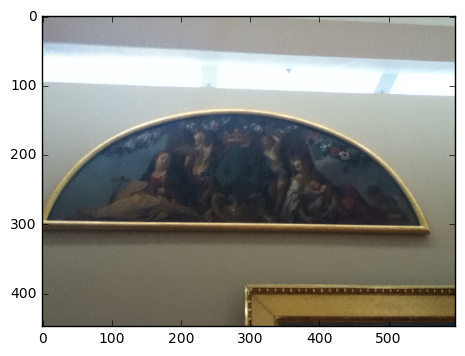
\includegraphics[width=\textwidth]{figures/sample1_10A-0519.png}
    %\caption{Image with label 10A\label{fig:sample1_id}}
  \end{minipage} \hfill
  \begin{minipage}[c]{.33\linewidth}
    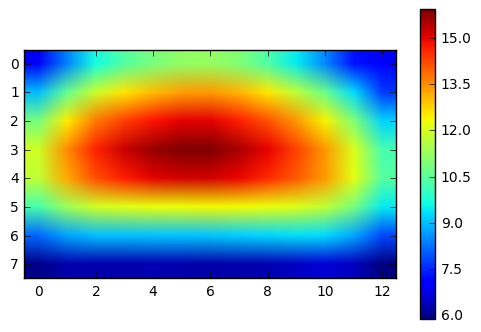
\includegraphics[width=\textwidth]{figures/sample1_heatmap.png}
    %\caption{Heat-map for 10A\label{fig:sample1_hm}}
  \end{minipage} \hfill
  \begin{minipage}[c]{.32\linewidth}
    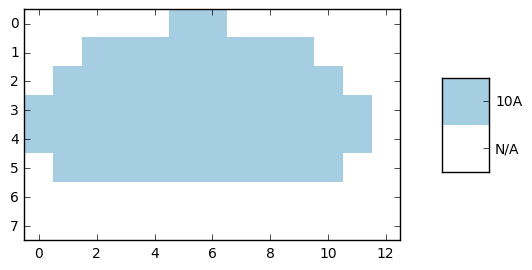
\includegraphics[width=\textwidth]{figures/sample1_labels.png}
    %\caption{Label-map for 10A\label{fig:sample1_lab}}
  \end{minipage}

  \begin{minipage}[c]{.33\linewidth}
    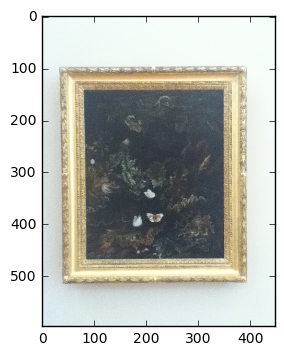
\includegraphics[width=\linewidth]{figures/sample2_5P-0508.png}
    %\caption{Image with label 5P\label{fig:sample2_id}}
  \end{minipage} \hfill
  \begin{minipage}[c]{.33\linewidth}
    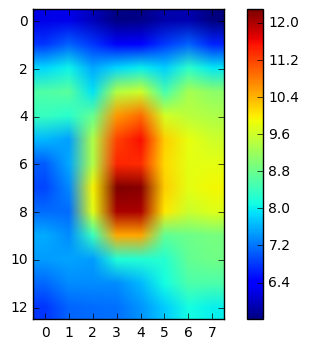
\includegraphics[width=\linewidth]{figures/sample2_heatmap.png}
    %\caption{Heat-map for 5P\label{fig:sample2_hm}}
  \end{minipage} \hfill
  \begin{minipage}[c]{.32\linewidth}
    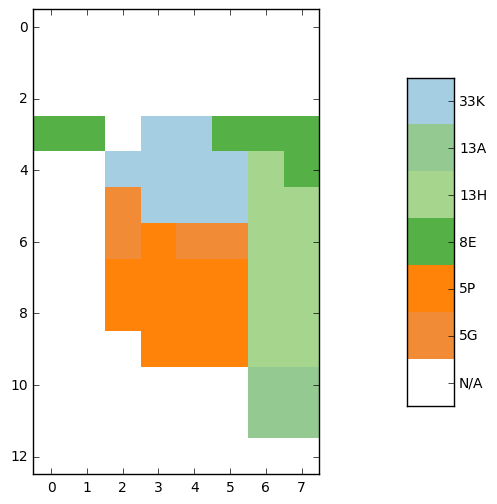
\includegraphics[width=\linewidth]{figures/sample2_labels.png}
    %\caption{Label-map for 5P\label{fig:sample2_lab}}
  \end{minipage}
  
  \begin{minipage}[c]{.33\linewidth}
    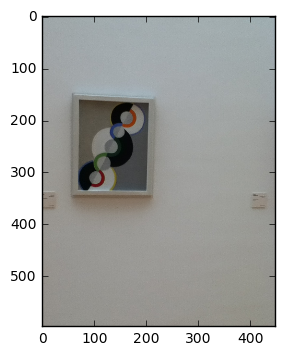
\includegraphics[width=\linewidth]{figures/sample3_30P-0976.png}
    %\caption{Image with label 30P\label{fig:sample3_id}}
  \end{minipage} \hfill
  \begin{minipage}[c]{.33\linewidth}
    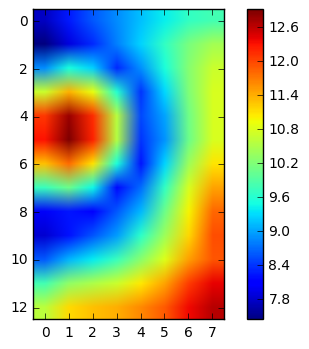
\includegraphics[width=\linewidth]{figures/sample3_heatmap.png}
    %\caption{Heat-map for 30P\label{fig:sample3_hm}}
  \end{minipage} \hfill
  \begin{minipage}[c]{.32\linewidth}
    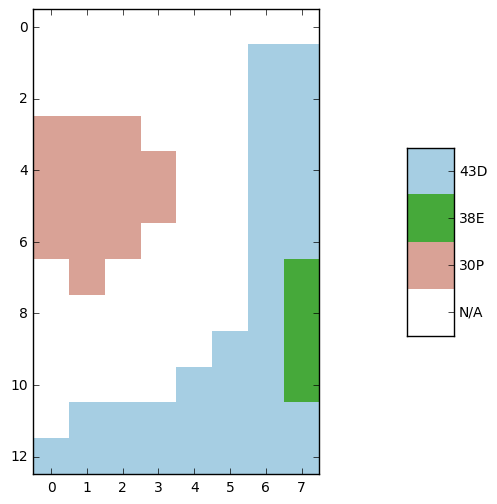
\includegraphics[width=\linewidth]{figures/sample3_labels.png}
    %\caption{Label-map for 30P\label{fig:sample3_lab}}
  \end{minipage}


	\caption{Exemple d'images avec les heat-map des activations maximales, obtenues à partir d'un ResNet-152 après un apprentissage fin. Le réseau est appliqué sur toute l'image de manière strié. Les labelles obtenu sur les zones d'activation maximales sont également indiqués.\label{fig:heatmaps}}
	
\end{figure}



\subsection{Apprentissage sur différentes régions}

Nous avons montré dans (section état de l'art), qu'un réseau entièrement convolutionel peut être appliqué sur une image quelque soit ça dimension. Cela permet d'appliquer un réseau de manière strié sur une grande image, sans faire plusieurs passage sur l'image.

Dans le but de faire un apprentissage fin, nous n'utilisons pas de réseau entièrement convolutionel, mais des CNN classique, avec couche de classification à la fin. Cependant, nous avons montré dans (section Etat de l'art) qu'il était possible de transformer une couche entièrement connecté, en une couche convolutionel. En utilisant cette méthode, il est possible d'obtenir les résultats présenté dans la figure~\ref{fig:heatmaps}, avec un réseau entièrement convolutionel.

Pour apprendre le réseau, nous utilisons le différentes échelles pour une image, et pour chaque échelle, différentes régions. La fonction de coût est calcul en moyennant l'entropie croisée, entre les régions, et entre les échelles. L'entropie croisée est calculée 


\begin{figure}
\centering
    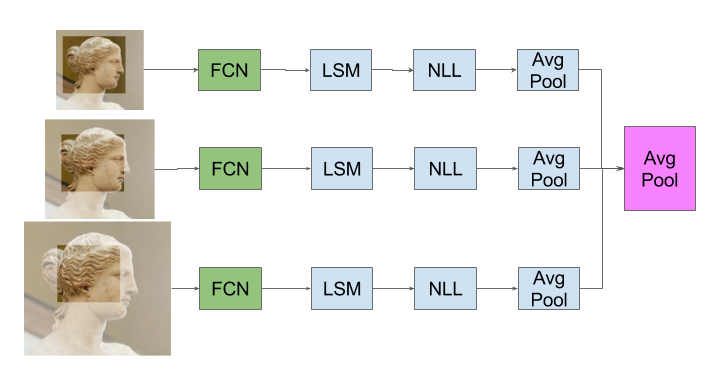
\includegraphics[width=\linewidth]{figures/Average_Loss.png}
    \caption{Calcul de la fonction de coût lorsque l'on entraine le réseau sur différentes régions à différentes échelles. LSM est le LogSoftMax et NLL le Negative Log-Likelihood. Il sont utilisés dans le calcul de la cross-entropy(eq.~\ref{eq:CE}).
    \label{fig:regionfinetuning}}
\end{figure}


\begin{equation}\label{eq:CE}
	\mathcal{CE}(x,y) = -y \log(softmax(x))
\end{equation}


\subsection{Apprentissage de régions et de similarité}


\begin{equation}\label{eq:fcnloss}
 \mathcal{L} = \frac{1}{S} \sum_{s=1}^S \frac{1}{H_s*W_s}
\sum_{h=1}^{H_s} \sum_{w=1}^{W_s} \mathit{CE}^{h,w}
\end{equation}


Dans l'équation~\ref{eq:fcnloss}, $S$ est le nombre d'échelles de l'image de départ.
$H_s$ et $W_s$ représentent la hauteur et la largeur de la carte de caractéristiques (feature-map), à une échelle $s$ données.
$CE^{h,w}$ représente la cross-entropie pour une région $(h,w)$.

\begin{figure}
    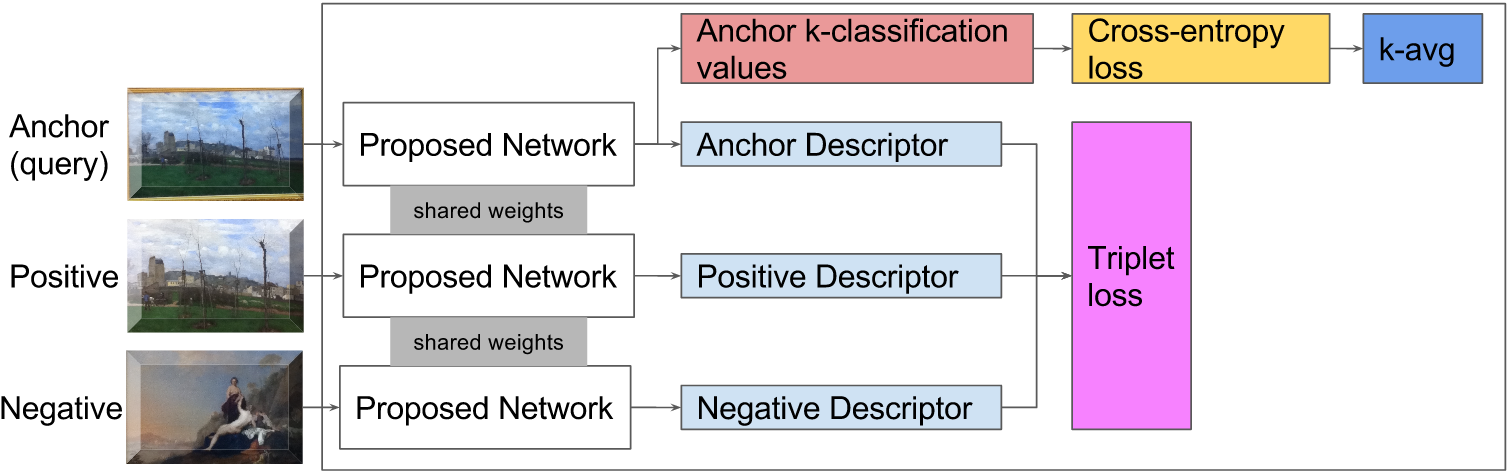
\includegraphics[width=\linewidth]{figures/contrib_train.png}
    \caption{Proposed architecture for instance search based on an FCN ~\cite{long_fully_2015} for region proposals, at training time
    \label{fig:contribtrain}}
%\caption{Proposed architecture for instance search, based on an FCN ~\cite{long_fully_2015} for region proposals.
%\label{fig:contrib}}
\end{figure}










\begin{figure}
\centering
    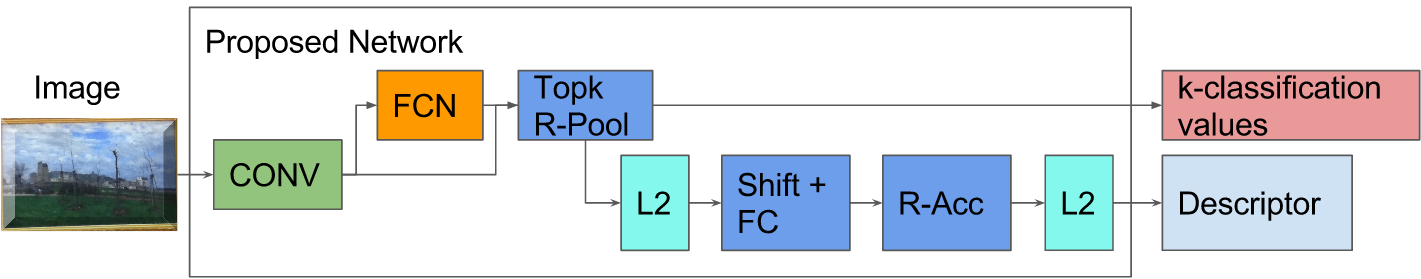
\includegraphics[width=\linewidth]{figures/contrib_deploy.png}
    \caption{Proposed architecture for instance search based on an FCN
~\cite{long_fully_2015} for region proposals, at deploy time
    \label{fig:contribdeploy}}
\end{figure}

\subsection{Évaluation}









